\subsection{Semantic Pixel Level Image Segmentation Task}
\label{sec:imseg}

With the knowledge of how neural networks perform their computation in general it is also necessary to think about how a specific task can be accomplished by crafting a specialized representation of the problem, which networks can be applied to.
There are several categories of typical problems within computer vision, that have different kinds of encodings for their solution space. The task which this thesis is trying to solve lies in the category of \emph{Semantic Pixel Level Image Segmentation}, where the network input is an image and the network is supposed to assign each pixel one of a predetermined set of \emph{classes} to which the object the pixel is part of belongs to. For example in the case of the \emph{Cityscapes Dataset}\cite{cordtsCityscapesDatasetSemantic2016a}, the data consists of images of inner city traffic situations from the perspective of a car, and the classes are subjects typically found in such scenarios like e.g. \emph{car}, \emph{road}, \emph{person}, \emph{building} etc.

\begin{figure}[htbp]
    \centering
    \begin{tabular}{ll}
        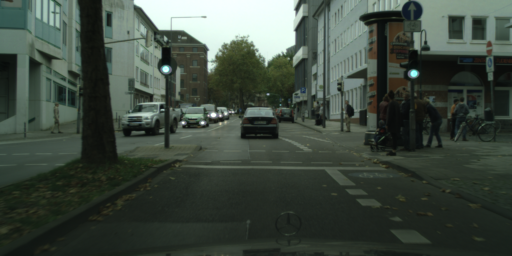
\includegraphics[width=0.45\textwidth]{images/aachen_000029_000019_leftImg8bit.png}
        &
        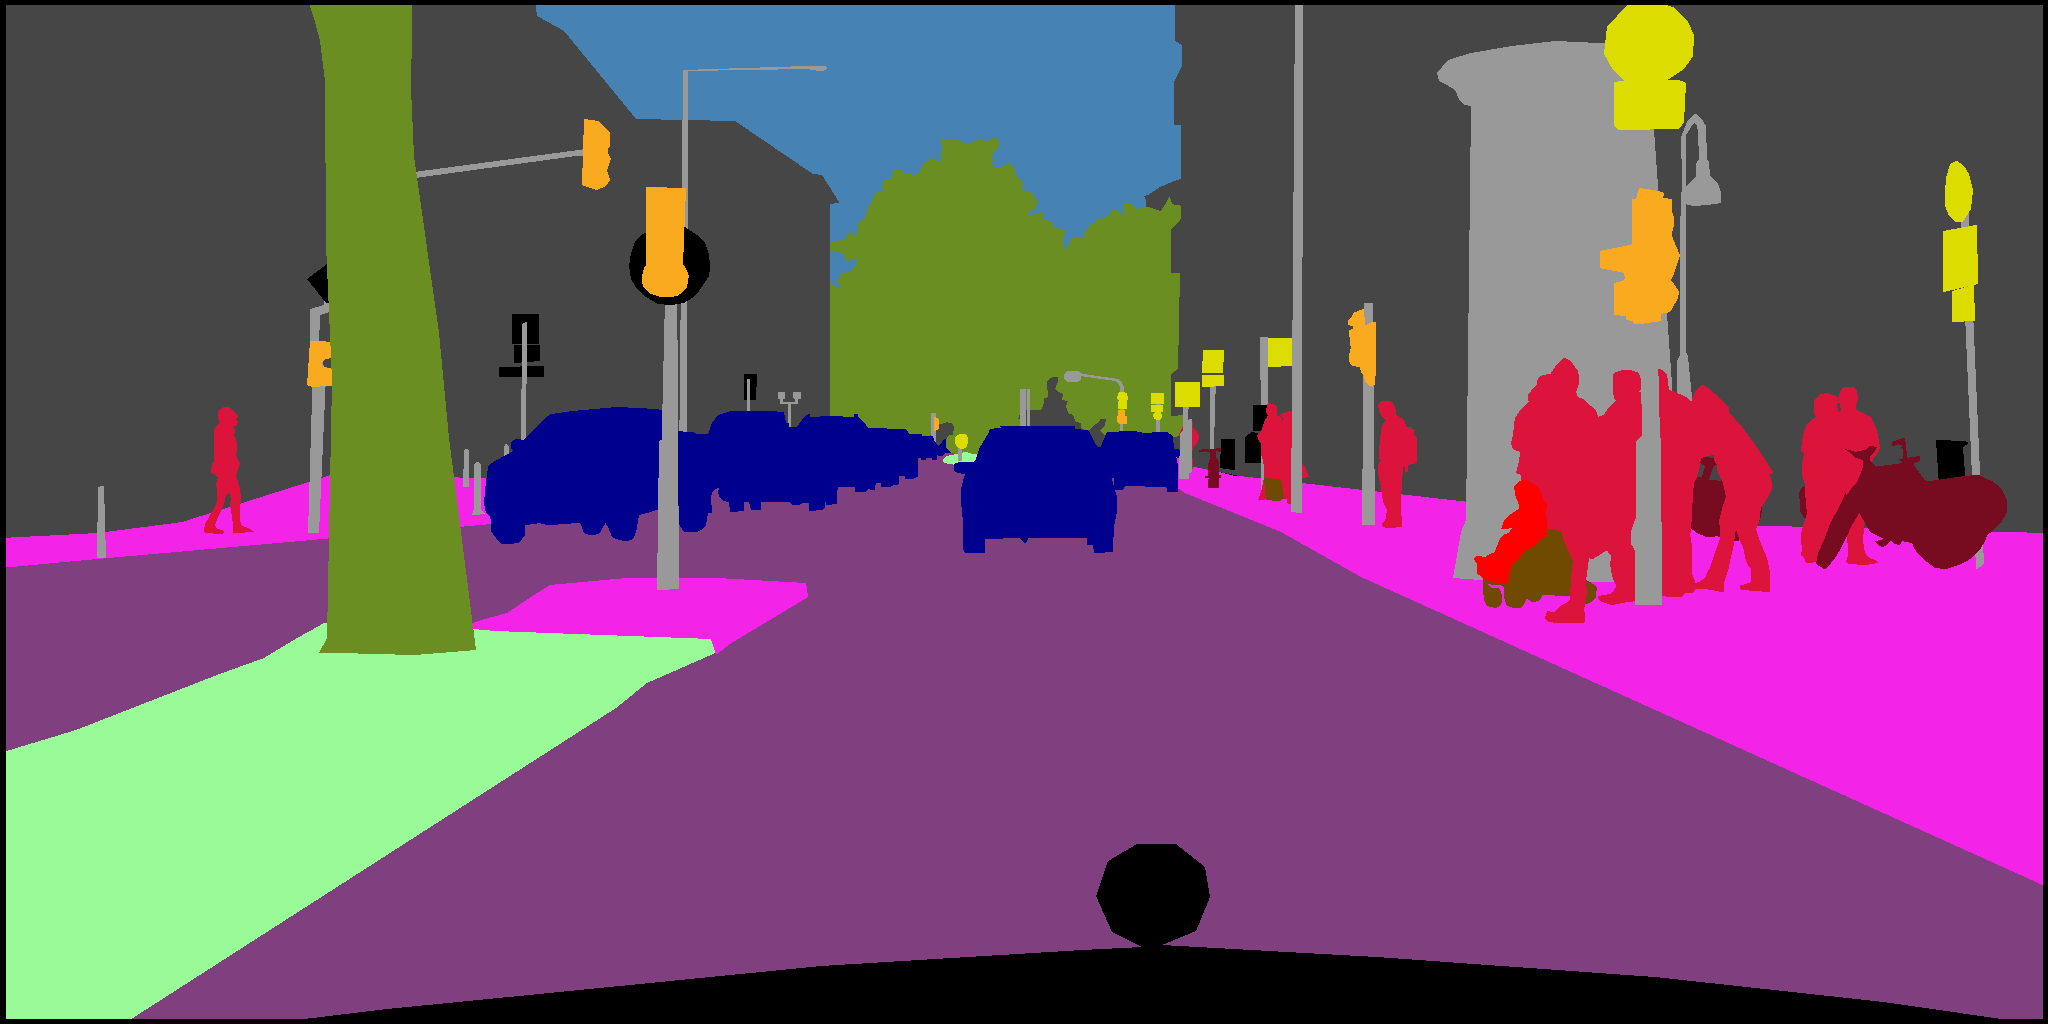
\includegraphics[width=0.45\textwidth]{images/aachen_000029_000019_gtFine_color.png}
    \end{tabular}
    \caption{A sample from the dataset \emph{Cityscapes}. On the left is the image that acts as an input for the network and on the right is the corresponding ground truth label mask showing different classes in different colors.}
    \label{fig:cityscapes_smpl}
\end{figure}

A model for this task would now output a map with the same spatial dimensions (e.g. $M\times N$) as the image and a number of channels $C$ equivalent to the number of possible classes. Each output pixel consists of a vector $\mathbf{x}\in \mathbb{R}^C$ where each entry $x_i$ corresponds to how much the network thinks the pixel belongs to class $i$. The channel with the highest value is the class the network has classified the pixel as.

These outputs can now be normalized to probabilities by applying the \emph{softmax} function to them or converted to a segmentation mask by using the \emph{argmax} function.

To evaluate how well a network performs on the segmentation task, the \emph{Intersection over Union} (IoU) for each class is computed, which if $A$ is the set of pixels labeled as a certain class by the network and $B$ the set of pixels which should actually belong to that class is calculated as follows:
$$
    \text{IoU} = \frac{\left|A\cap B \,\right|}{\left|A\cup B \,\right|}
$$
This metric is very informative to look at per class, but typically the mean over all classes (mIoU) is used to evaluate the model as a whole.\\

A big problem in developing AI solutions to this kind of task is its huge demand for varied data to train models on. High quality annotated data is very time and cost consuming to produce, for example according to the Cityscapes team, one annotated image such as seen in Figure \ref{fig:cityscapes_smpl} took \SI{90}{min} to create. 
Further in this thesis techniques to mitigate this problem and achieve good results on little annotated data will be discussed.
